\documentclass[letterpaper,10pt,titlepage]{article}

\usepackage{amsmath}                                         
\usepackage{amsthm}

\usepackage{alltt}                                           
\usepackage{float}
\usepackage{color}

\usepackage{balance}
\usepackage[TABBOTCAP, tight]{subfigure}
\usepackage{enumitem}

\usepackage{pstricks, pst-node}
\usepackage{geometry}
\geometry{textheight=10in, textwidth=7.5in}
\usepackage{graphicx}
%random comment

\newcommand{\cred}[1]{{\color{red}#1}}
\newcommand{\cblue}[1]{{\color{blue}#1}}

\usepackage{hyperref}

\def\name{David Merrick}


%% The following metadata will show up in the PDF properties
\hypersetup{
  colorlinks = true,
  urlcolor = black,
  pdfauthor = {\name},
  pdfkeywords = {cs311 ``operating systems'' pipes signals},
  pdftitle = {CS 311 Project 3: Uniqify},
  pdfsubject = {CS 311 Project 3},
  pdfpagemode = UseNone
}

\parindent = 0.0 in
\parskip = 0.2 in

\begin{document}
David Merrick

CS 311

15 February, 2013

\begin{center}
{\LARGE Writeup for Assignment 3}
\end{center}

\begin{enumerate}

\item \emph{Plots}
\begin{figure}[H]
	\begin{center}
	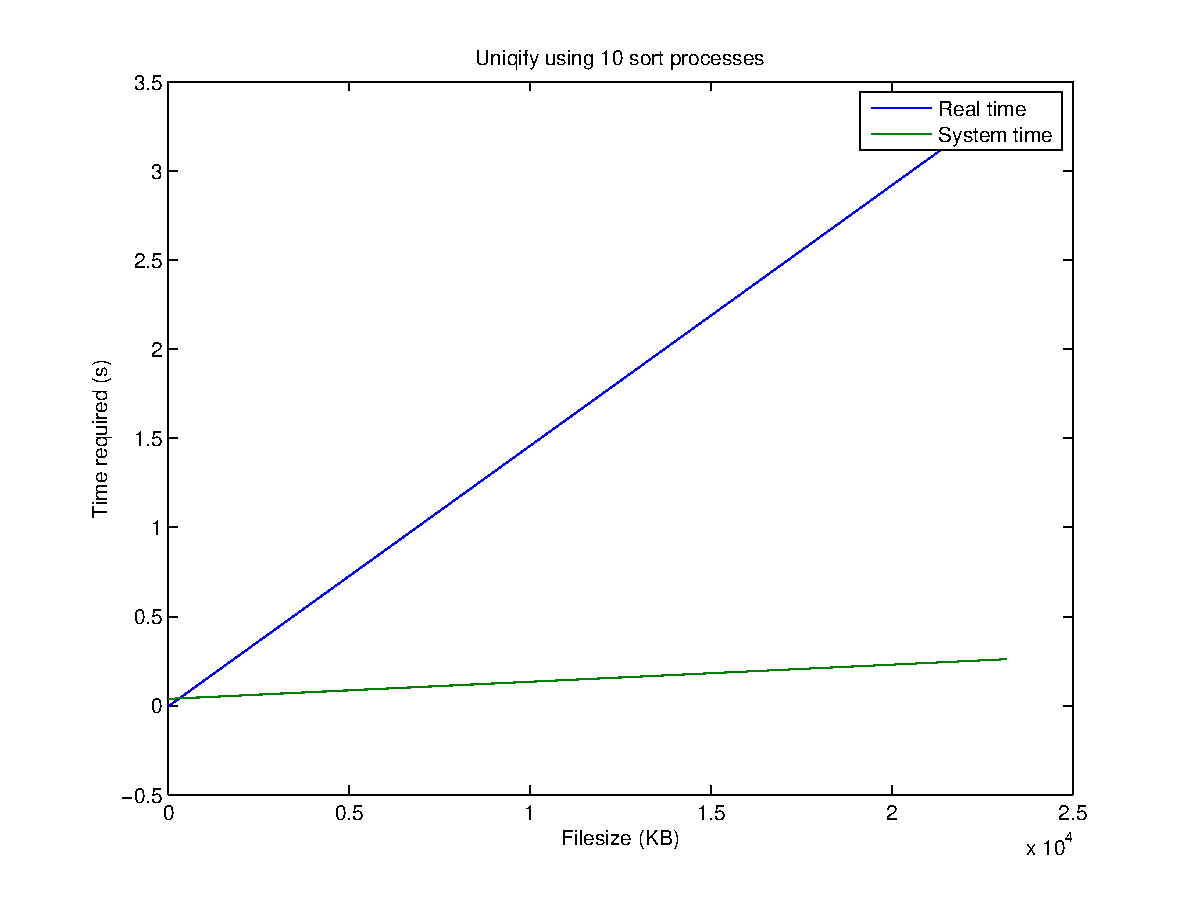
\includegraphics[width=8in]{figure1}
	\end{center}
	\caption{Uniqify using 10 sort processes.}
\end{figure}
\begin{figure}[H]
	\begin{center}
	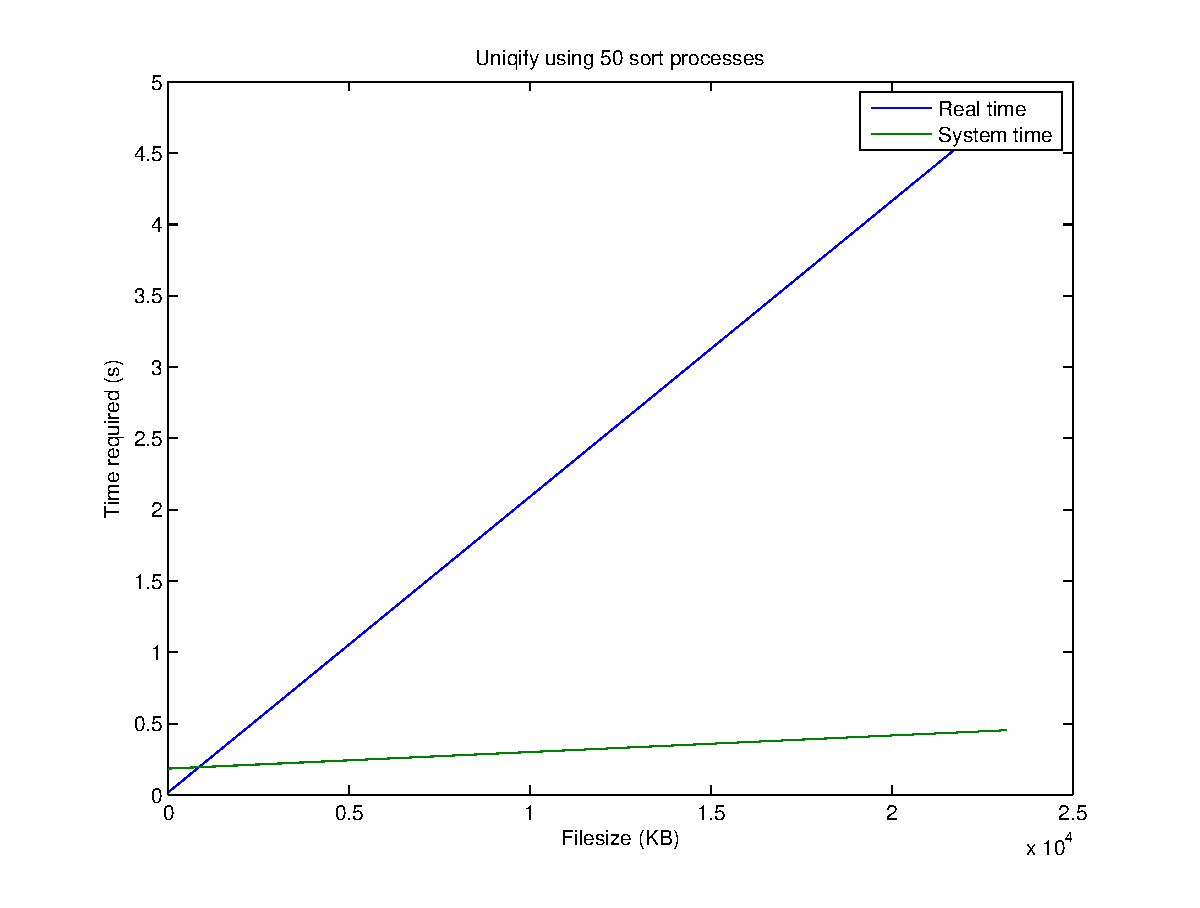
\includegraphics[width=8in]{figure2}
	\end{center}
	\caption{Uniqify using 50 sort processes.}
\end{figure}
\begin{figure}[H]
	\begin{center}
	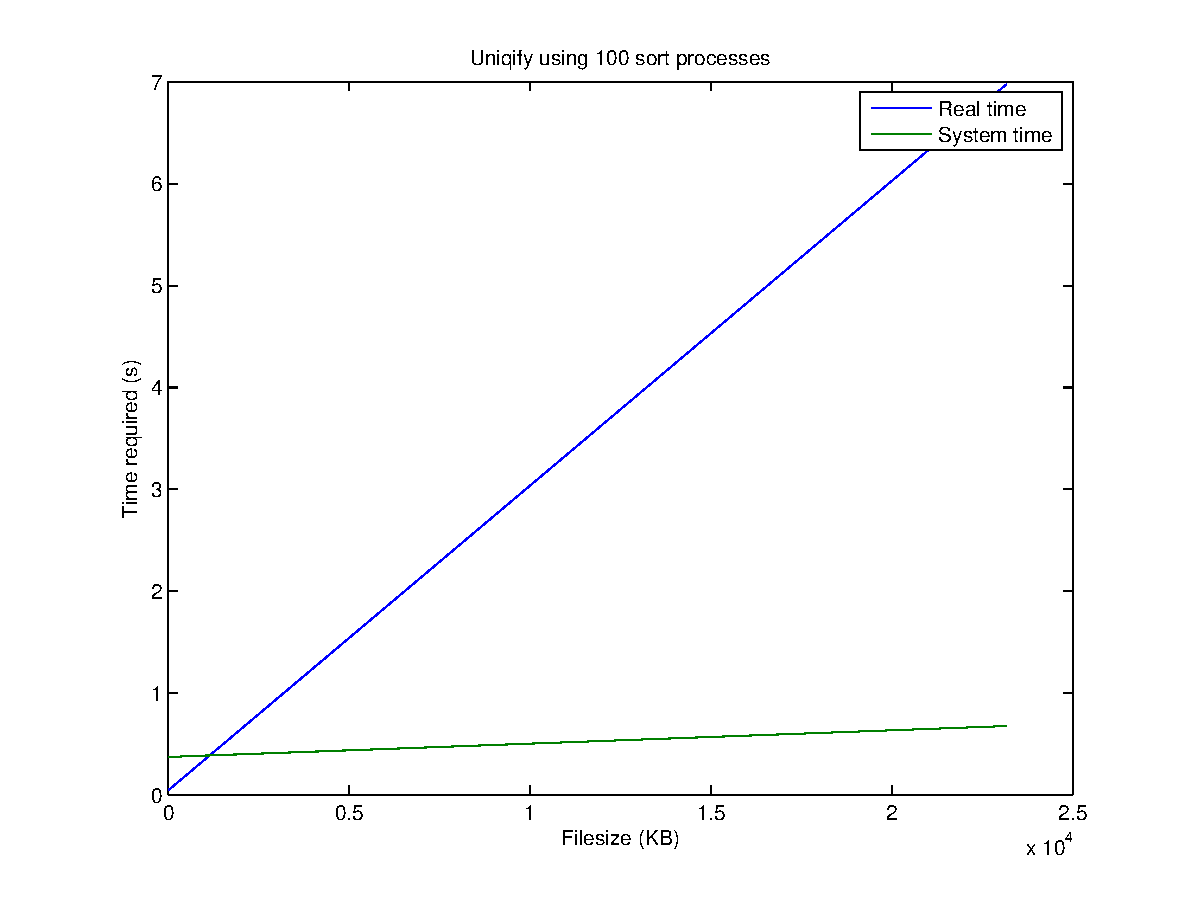
\includegraphics[width=8in]{figure3}
	\end{center}
	\caption{Uniqify using 100 sort processes.}
\end{figure}

\item \emph{A design for your system, as well as places your implementation deviated from this design.}
I designed my system to be as efficient as possible and to minimize rewriting code by substituting functions wherever I had repetition. Initially, I deviated from this in a couple of places. In the parser, I was reading in one character at a time, writing a null termitator character to the end of the buffer, then writing one character at a time to the pipes. This obviously was not an optimal way to read input, so later I switched to using scanf to read an entire word at a time and then write that. Initially, I was opening an entire array of pipes in the parent, then looping through in the parent and the child closing the ones I didn't need. I switched this to opening only the pipes I needed where I needed them. I still had to loop through and close the previous children's pipes in the subsequent children (because those pipes were inherited by the parent), but there was no other more efficient way to do this that I was aware of. Initially, my suppressor process was not optimal. I read words into an array, performed an insertion sort, returned the array, then printed them. Not only was this a waste of time, but it didn't output the words in the right order. It couldn't. Not without reading every word into an array from the pipes. So instead, I switched to a function that found the next highest alphabetical word from each pipe and stored it in a struct that kept track of its count. It repeated this until there were no more words, and printed out words plus counts when it found new ones. This minimized the use of memory, made it unnecessary to perform a bunch of insertion sorts, and worked in every case. 

\item \emph{Work Log:}

2013-02-15 10:15:43 -0800, Tweaked parser to read and discard leading nonalpha chars.

2013-02-14 15:13:06 -0800, Changed parser to use scanf.

2013-02-14 14:56:24 -0800, Fixed bug. Wasn't closing certain pipes in children, causing program to hang. Works now. Now just need to improve parser.

2013-02-14 11:20:14 -0800, This version of code is NOT working. Saving it here so I can revert to earlier version and see what went wrong.

2013-02-14 10:57:38 -0800, Reverted back to old suppressor. still weird bug

2013-02-13 16:06:57 -0800, Found a bug where it hangs on fgets in the suppressor sometimes. I couldn't figure out why. Will ask. Also added scanf to parser, which fixed the problem of blank lines in output.

2013-02-13 13:47:34 -0800, Tweaks and indenting.

2013-02-13 13:43:57 -0800, Updated parser to use fgets.

2013-02-13 13:16:50 -0800, Redid signal handling. Much cleaner now because it doesn't send a QUIT signal to itself.

2013-02-13 12:24:59 -0800, Removed camelcasing from variables.

2013-02-13 09:05:45 -0800, Fixed bug where it wasn't printing the last word

2013-02-12 21:13:51 -0800, Added code to free malloced arrays for pipes at the end to fix memory leak.

2013-02-12 16:31:15 -0800, Added helpful error message if number of pipes is OVER 9000git add uniqify.c

2013-02-11 20:42:19 -0800, Changed syntax of printed words to match uniq -c

2013-02-11 20:29:25 -0800, Added proper indentation with indent -kr -i8 [filename] command

2013-02-11 20:17:09 -0800, Setup signal handlers. They seem to be working to spec but will double-check. Removed unneccessary typecasting from malloc() statements. Code seems done and bug-free

2013-02-11 17:09:46 -0800, Patched bug with a couple lines of code. Still would like to know why it's happening. Other than that, just need to handle signals and am done with the program

2013-02-11 16:37:43 -0800, Updated code so it spawns suppressor process instead of calling it from parent.

2013-02-11 16:26:39 -0800, Code is all working except for slight bug. I think bug is in parser. Results in pipe initially being empty

2013-02-11 15:21:01 -0800, Program works, but my solution was a little hackish and might not work for all cases. Maybe should ask if there's a better way.

2013-02-11 10:43:37 -0800, It's mostly working! There's just a slight bug in the printWords function where it doesn't pick up on duplicate words or count them sometimes.

2013-02-11 09:43:44 -0800, Suppressor is currently broken. About to do some major work to fix but am committing what I have now.

2013-02-10 18:13:12 -0800, Debugging suppressor process. MergeWords seems to be working at alphabetizing words. But keep getting segfaults. Will debug later.

2013-02-10 13:37:31 -0800, Started work on mergeWords function. It's a little buggy and maybe inefficient but I can refine it later.

2013-02-10 12:40:06 -0800, Nvm, got it working. Had to close output pipes in parent.

2013-02-10 12:29:21 -0800, Trying to debug suppressor process. Weird behavior. Hangs in while loop.

2013-02-10 11:15:48 -0800, Finally fixed bug! Problem was that I was creating pipes when I was making the pipes array. Not sure why this was an issue but is fixed now. Removed debug functions.

2013-02-09 23:43:48 -0800, Added readme files to provide instructions and context for assignments

2013-02-09 23:41:47 -0800, instructions for first assignment

2013-02-09 22:29:39 -0800, Used write() instead of fputs() to put text into pipes. It's still acting weird and hanging with more than 2 processes.

2013-02-09 20:55:52 -0800, Added debug methods. Still acting weird and I'm not sure why. Throws bad file descriptor error with one process, hangs on more than one process.

2013-02-09 17:29:04 -0800, Made a few tweaks. Same thing is happening with processes greater than 1.

2013-02-09 16:10:08 -0800, Rewrote pipes to use a 2-dimensional array for easier coding and fewer counter variables.

2013-02-09 15:31:11 -0800, Is working except sort processes are not dying when numsort > 2. Strangely, if I kill any one process, they all die. Pipes are working correctly. Not sure where the bug is.

2013-02-09 00:01:21 -0800, Fixed warnings about fdopen(). Added wait at the end of main process to reap zombies.

2013-02-08 20:33:46 -0800, Added suppressor. Still doesn't print to STDOUT in my terminal but I think all the pipes are working.

2013-02-08 16:20:55 -0800, sort is working with multiple child processes

2013-02-08 15:44:34 -0800, Added code for suppressor pipes. But not working. So gonna revoke. But wanted to save on here.

2013-02-08 13:48:46 -0800, Trying to close write ends of pipes but not working. Made some other tweaks. Hangs on waits so gotta fix that.

2013-02-08 12:56:19 -0800, Sorting works! If there's only one subprocess

2013-02-08 12:34:57 -0800, Started work on multiple process children, successfully parsed input, child sort processes not working yet

2013-02-08 09:21:20 -0800, Successfully got a single sort pipe sorting output

2013-02-06 19:56:51 -0800, Added help function. parsing input isn't working but am gonna skip that for now and assume input is in csv format

2013-02-06 09:43:57 -0800, Version one of uniqify


\item \emph{Challenges:}
One major challenge of this program was to make sure the pipes were set up correctly. I decided the best approach to this would be iterative; First open pipes and create a subprocess that prints everything in them, then bind the pipes to the child's STDIN and exec the sort processes and make sure the output is correct, then bind the pipes in the children to STDOUT and make sure that output is correct. This was much easier said than done, and even after I thought I had it working 100 percent, I had forgotten to close the previous children's pipes in the subsequent children. Several frustrating hours of testing later, I realized this and corrected it. Another challenge was in debugging the child supressor process. I was initially not sure how to get GDB to follow the fork to the child, so I wrote a separate function, debugged it, then just had the child call that function after the fork. Another challenge was signal handling. I wasn't sure how to have the main program send a QUIT signal to all the children, because the signal handler is not able to access a local variable that held the child PIDs. But I realized that I could create a global array variable to keep track of each child then issue a QUIT to each one of them within the signal handler.

\item \begin{enumerate}
	\item \emph{What do you think the main point of this assignment is?} The main point of this assignment was to get familiar with interprocess communication and signal handling. Besides those two challenges, the rest of the program was just C and a little file I/O, which we already knew how to do.

	\item \emph{How did you ensure your solution was correct?}
I ensured my solution was correct by testing it on small files that I knew the word count of. I made sure every word was unique and had the correct count associated with it. Then I tested it on larger files with weird characters to see if it could handle them. Then I changed the number of sort processes I wanted it to use and repeated this process.

	\item \emph{What did you learn?}
I learned how to use GDB to debug child processes, how to use global variables, how to parse text using scanf, how to handle signals, how to spawn child processes, how to create zombies if you're not careful waiting for child processes, how to write to pipes, and how to read from pipes. I also learned that no matter how sure you are a part of your program works correctly, it can still have a bug.
	\end{enumerate}
\end{enumerate}

%input the pygmentized output of mt19937ar.c, using a (hopefully) unique name
%this file only exists at compile time. Feel free to change that.
%\input{__mt.h.tex}
\end{document}
